%=========================================================================
% (c) 2011, 2012 Josef Lusticky

\chapter{Analysis}
For implementation of a reasonably useful NTP client,
an operating system must be able to set, get and eventually adjust the system time.
Though not mandatory, adjusting the time is an important function,
if the time shall be always a monotonically increasing function.
Apart from that, ability to communicate over UDP is also required.

For developing and testing Contiki NTP Client,
the AVR Raven platform with 8-bit ATmega1284P CPU~\cite{avr-datasheet} will be used.
This platform features IEEE~802.15.4 (Low-Rate Wireless Personal Area Networks) link layer support.
Together with an adaptation layer called 6LoWPAN (IPv6 over Low power Wireless Personal Area Networks),
AVR Raven is able to communicate over IPv6.

%=========================================================================
% (c) 2011, 2012 Josef Lusticky

\section{Time interface}\label{sec:analysis-time}
For keeping, measuring and resolving the time computer needs a clock.
A computer clock is an electronic device with a counter register counting oscillations in a
quartz crystal oscillator with a particular frequency~\cite{thesis-sync}.
The structure of the clock hardware is shown in figure~\ref{fig:system-hardware-clock}.
\begin{figure}
  \centering
  
\includegraphics[width=9cm,keepaspectratio]{fig/pc-clock.png}
  \caption{A typical hardware clock (source:~\cite{thesis-beat})}
  \label{fig:system-hardware-clock}
\end{figure}
When the counter reaches a specific value, an interrupt is generated and the counter register is reset.
Such interrupt is called {\it{clock tick}}, or {\it{timer tick}}, and at each clock tick,
interrupt service routine increments a system clock value stored in the memory~\cite{thesis-sync}.
In a typical computer clock design, interrupts are produced at
fixed tick intervals in the range 1-20~ms~\cite{nanokernel}.

In Contiki, such a design is used by the clock library, described in section~\ref{sec:contiki-timers}.
There is a variable counting clock ticks, called {\it{scount}},
and a variable counting seconds, called {\it{seconds}}.
As described in section~\ref{sec:contiki-timers}, there are
exactly {\it{CLOCK\_SECOND}} ticks in one second.
When the {\it{scount}} variable reaches this value,
the {\it{seconds}} variable is incremented and the {\it{scount}} variable is reset.
Both variables are used by the Contiki timers discussed in section~\ref{sec:contiki-timers}.

Since the value of the {\it{seconds}} variable is zero after the system booted,
it actually expresses the system uptime.
The {\it{seconds}} variable can be read by the application using the {\it{clock\_seconds}} call.
However, in Contiki 2.5 there is no call for setting this variable.
In the current Git version at the time of writing, a new call {\it{clock\_set\_seconds}}
can be used for this purpose.
Because this call simply rewrites the {\it{seconds}} variable, it breaks the stimer library,
and should by avoided by the NTP client.
%The {\it{clock_set_seconds}} call is implemented only for three CPU architectures at the time of writing.

The precision of one second is also not adequate for the NTP client.
Further precision can be acquired by reading the {\it{scount}} variable,
as it provides resolution of $\frac{1}{CLOCK\_SECOND}$.
Moreover, the hardware counter can be also queried, as it includes the time passed since
the last update of the {\it{scount}} variable.
If stimers should not be broken by setting the {\it{seconds}} variable,
and Contiki should be able to set and provide the current time in a higher precision,
a new call interface must be developed.

Similarly, there is no call for adjusting the time in Contiki.
Due to memory constraints, software structures controlling the time adjustments are too heavyweight
for a usage in an embedded operating system.
Due to lower CPU frequencies, the code of an interrupt service routine can not be complex
and sophisticated clock discipline algorithms should be avoided.
Because of this, a call for adjusting the time should use abilities
provided by the hardware clock as much as possible.


%=========================================================================
% (c) 2011, 2012 Josef Lusticky

\section{Clock subsystem}\label{sec:analysis-clock}
Contiki provides a basic clock interface particularly for use of timers
with a simple goal - measuring time.
This interface is common for all supported platforms,
but the particular implementation is platform specific.
The definition of the common interface is located in the {\it{core/sys/clock.h}} file
and the specific implementations can be found in the {\it{clock.c}} file
in {\it{cpu/}} directory of the Contiki source code.

The clock interface provides the {\it{clock\_init}} call for initialising the hardware clock,
that is automatically called during the boot sequence of Contiki.
The {\it{clock\_init}} call sets up
appropriate registers and the interrupt service routine as described in section~\ref{sec:analysis-clock}.
This call is implemented as the C macro for AVR CPUs, that evaluates to a specific setup code for each
different AVR CPU during the compilation, and is defined in the {\it{cpu/avr/dev/clock-avr.h}} file.
The setup code is not common to all AVR CPUs because of differences among them - e.g. there are usually
only three Timer/Counter modules, but AVR ATmega1284P has four Timer/Counter modules~\cite{avr-datasheet}.

On AVR Raven, 8 bit Timer/Counter~2 clocked from asynchronous 32~768~Hz crystal oscillator
is used by default by Contiki clock interface.
This oscillator is independent of any other clock,
can be only used with Timer/Counter~2 and it
enables use of Timer/Counter~2 as a Real Time Counter~\cite{avr-datasheet}.
The Timer/Counter~2 prescale value 8 is used in Contiki on AVR Raven platform -
the oscillator frequency of 32~768~Hz is effectively divided by 8.
The counter register is hence incremented with the frequency of
$f_{T2} = {\frac{f_{asy}}{prescaler}} = {\frac{32768}{8}} = 4096$~Hz.
Figure~\ref{fig:avr-clock} shows the Timer/Counter~2 clock module.
\begin{figure}
  \centering
  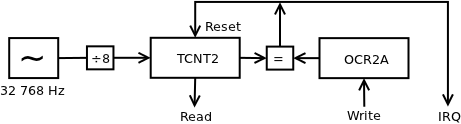
\includegraphics[width=9cm,keepaspectratio]{fig/avr-clock.png}
  \caption{Timer/Counter 2 hardware clock module on AVR Raven}
  \label{fig:avr-clock}
\end{figure}

%%Unlike I/O clock used for clocking other Timers/Counters,
%%this asynchronous crystal is also active in power-save mode~\ref{avr-datasheet}.
%CITATION: If Timer/Counter2 is enabled, it will keep running during sleep. The device can wake up from
%either Timer Overflow or Output Compare event from Timer/Counter2.
%If Timer/Counter2 is not running, Power-down mode is recommended instead of Power-save
%mode.
%The Timer/Counter2 can be clocked both synchronously and asynchronously in Power-save
%mode. If the Timer/Counter2 is not using the asynchronous clock, the Timer/Counter Oscillator is
%stopped during sleep. If the Timer/Counter2 is not using the synchronous clock, the clock source
%is stopped during sleep. Note that even if the synchronous clock is running in Power-save, this
%clock is only available for the Timer/Counter2.

The Timer/Counter~2 module is used in the Clear Timer on Compare Match (CTC) mode by Contiki.
In this mode, the counter register {\it{TCNT2}} is incrementing
and the compare register {\it{OCR2A}} defines the maximum value of the counter register.
Compare match between the counter register and the compare register
sets the Output Compare Flag {\it{OCF2A}} and resets the counter register to zero~\cite{avr-datasheet}.
This behaviour is illustrated in figure~\ref{fig:design-timing-diagram}
- the {\it{TOP}} value is equal to the value in the compare register and the {\it{BOTTOM}} value is equal to zero.

\begin{figure}
  \centering
  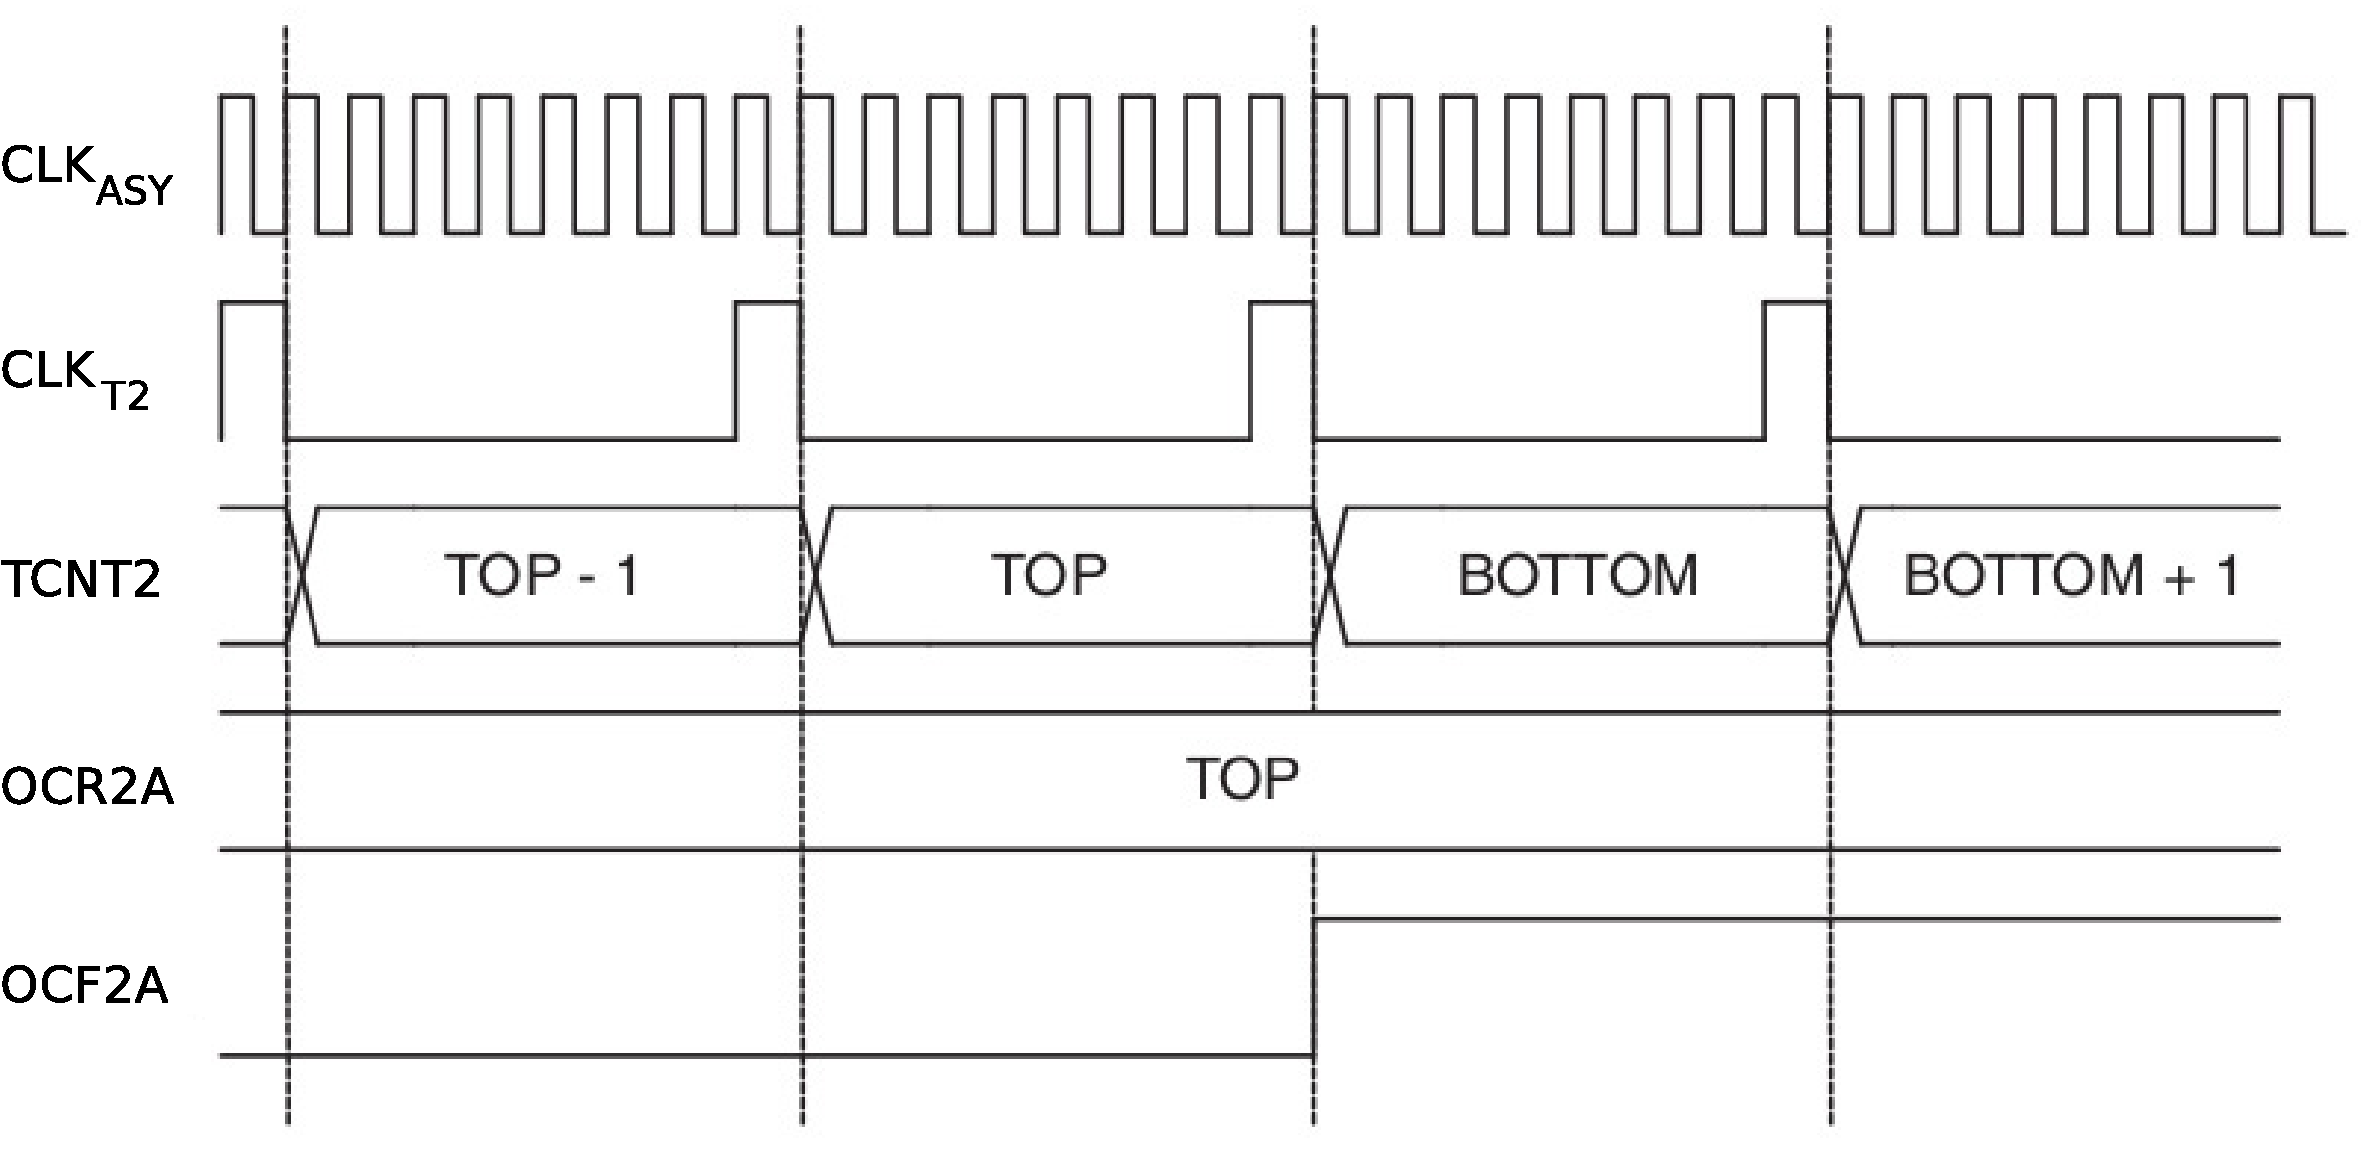
\includegraphics[width=12cm,keepaspectratio]{fig/timing-diagram.pdf}
  \caption{Timing diagram in CTC mode with prescaler 8 (source:~\cite{avr-datasheet})}
  \label{fig:design-timing-diagram}
\end{figure}

Additionally, when compare match occurs,
an interrupt is raised and the interrupt service routine {\it{AVR\_OUTPUT\_COMPARE\_INT}},
defined in {\it{cpu/avr/dev/clock.c}} file, is executed.
The flag indicating occurred match {\it{OCF2A}} is
cleared automatically by hardware when executing
the interrupt service routine in this case~\cite{avr-datasheet}.

To obtain {\it{CLOCK\_SECOND}} interrupts per second, there must be
${\frac{f_{T2}}{CLOCK\_SECOND}}$ hardware clock ticks between two successive interrupts.
On compare match in CTC mode, the timer is reset to zero as
shown in figure~\ref{fig:design-timing-diagram}.
The value zero is also included in the counting - the 0th count of the timer also takes one tick.
Therefore the value of compare register {\it{OCR2A}} must be ${\frac{f_{T2}}{CLOCK\_SECOND}} - 1$
when using Timer/Counter~2 in CTC mode.
The default value of {\it{CLOCK\_SECOND}} for AVR Raven in Contiki is 128,
which implies the default value of the compare register ${\frac{4096}{128}} - 1 = 31$.
The {\it{CLOCK\_SECOND}} value is defined in {\it{platform/avr-raven/contiki-conf.h}} file
and the default value of the compare register is computed during the compilation.

The interrupt service routine can be further used for updating the value in {\it{OCR2A}} compare register.
This can be used for adjusting the time, because decrementing the compare register
value causes a faster increment of the {\it{scount}} variable, which in turn causes
a faster increment of the {\it{seconds}} variable and vice versa.
However, changing {\it{OCR2A}} to a value closer to zero when the counter is running
must be done with care since the CTC mode does not have a double buffering feature.
If the new value written to {\it{OCR2A}} is lower than the current
value of {\it{TCNT2}}, the counter will miss the compare match~\cite{avr-datasheet}.



\section{Communication}
Without any NTP server is an NTP client useless. % There are clients, servers...
However, too many server associations complicate the client design.
In fact, in the most common scenario, there can be only a single NTP master server
for the whole network.
A single server association requires just a simple calculation of the local clock offset
$\theta$, whereas more server associations require the intersection algorithm,
described in section~\ref{sec:ntp-algorithms}.
Implementation of such an algorithm, requiring advanced data structures, should be avoided
in a memory constrained system.

The NTP broadcast communication mode, on the other hand,
requires no associations and no packet filling process on the client side.
Moreover, because the client does not have to actively send any NTP packets,
an energy consumption of the client is reduced.

% 1 - see design
A problem might be a possible packet loss when communication uses UDP on transport layer.
The reason why this can happen often in Contiki, is explained in section~\ref{sec:contiki-uip}.
% 2
In NTP unicast mode, the packet loss might occur either for a client's query to the server
or for a server's response to the client.
If the client's query loss occurs, no server response will be sent.
Similarly, if the server's response loss occurs, no message will be received by the client.
Not to block a whole system till the response arrives
is therefore a desired behaviour of the client.

The NTP client should be able to communicate over both IPv4 and IPv6.
Thanks to the uIP stack, this is no a matter for Contiki.
The only constraint is that both IP versions can not be used simultaneously
and the decision must be made during the compilation~\cite{contiki-docs}.
Although the {\it{UIP\_CONF\_IPV6}} macro can be used to determine which IP version
support is being compiled, the NTP client application can be written IP-version agnostic.


\section{Timestamp conversions}%CLIENT CODE
As mentioned in section~\ref{sec:ntp-time}, the NTP timescale is not
coincident with the POSIX timescale.
If the new call interface should use the standard POSIX timescale,
conversion between NTP and POSIX timestamps must be calculated.
The conversion from the POSIX timestamp to the 64-bit long NTP timestamp
is needed when the client sends the request
and the conversion vice versa is needed when the client calculates
the local clock offset from the received timestamps.

Since both timescales reckon in seconds, the conversion between
the NTP timestamp seconds field value and the POSIX timestamp seconds field value is simple.
However, the conversion between the NTP fraction field value ($2^{-32}$)
and the POSIX fraction field value (nanoseconds or microseconds) is problematic.
The relation between the POSIX fraction field and the NTP fraction field
is given by $POSIX.frac = NTP.frac \times POSIX.res \div 2^{32}$,
where $POSIX.frac$ is the POSIX fraction field value,
$NTP.frac$ is the NTP fraction field value and
$POSIX.res$ is the POSIX timestamp resolution (microseconds or nanoseconds).
The accurate conversion requires either floating point operations or operations with 64 bit numbers.
These operations can be memory expensive, especially on 8-bit microcontrollers,
and their usage must be considered carefully or another suitable solution must be found.


%Operating system maintains the current time and advances it at every interrupt.



%Such a design is also used by the timer library in Contiki~\cite{contiki-docs}.

%Because of the speed requirement,
%the system time uses a linear time scale like seconds
%(instead of dealing with seconds, minutes, hours, days, etc.)
%and only if a human is in need of the current time,
%the system time is converted~\cite{ntp-faq}.




%\section{Clock quality factors}
%Unfortunately all the common clock hardware is not very accurate~\cite{ntp-faq}.
%This is simply because the frequency that makes time increase is never exactly right.
%Even an error of only 0.001\% would make a clock be off by almost one second per day.
%Almost every clock can have unique behaviour depending on many conditions~\cite{ntp-faq}.
%The following factors are therefore used for expressing clock quality and behaviour:
%\begin{itemize}
%\item
%Frequency is the rate at which a clock progresses~\cite{thesis-sync}.
%\item
%It is sometimes convenient
%to express frequency offsets in parts-per-million~(PPM), where~1~PPM
%is equal to $10^{-6}$ $\frac{s}{s}$ (0.0001\%)~\cite{rfc5905}.
%\item
%From long-term observation one may also notice variations in the clock frequency.
%The difference of the frequency is called wander~\cite{ntp-faq}.
%There can be clocks with poor short-term stability, but with good long-term stability, and vice versa.
%\item
%Resolution is the smallest possible increase of time the clock model allows.
%If a clock increments its value only once per second, its resolution is also one second~\cite{ntp-faq}.
%\item
%Precision is the smallest possible increase of time that can be experienced
%by a program~\cite{ntp-faq}.
%\item
%When repeatedly reading the time, the difference may vary almost randomly.
%The difference of these differences (second derivation) is called jitter~\cite{ntp-faq}.
%\item
%Accuracy determines how close the clock is to an official time reference~\cite{ntp-faq}.
%\item
%Offset is the difference between the time read by the clock and the reference time~\cite{thesis-sync}.
%\item
%Reliability determines the time a clock can keep within a specified accuracy~\cite{ntp-faq}.
%\end{itemize}

%As mentioned before, all of the common hardware clocks are not very accurate.
%Real clocks have a frequency error of several PPM quite frequently
%and some of the best clocks available still have errors of about $1^{-8}$PPM~\cite{ntp-faq}.
%Even if the systematic error of some clock model is known, the clock will never be perfect.
%This is because the frequency varies over time, mostly influenced by temperature,
%but it could also be air pressure or magnetic fields~\cite{ntp-faq}.

%\section{Clock discipline}\label{sec:system-discipline}
%For keeping an accurate time a clock not only needs to be read, it must be also set.
%However, simply setting the clock to remove the offset would cause unpredictable time steps~\cite{ntp-faq}.
%Since real time is an always monotonically increasing function, this is not a desired behaviour~\cite{ntp-faq}.
%For minimising the time offset and frequency difference between
%the reference clock and the local clock without any time step, an NTP client can be used.

%With the current system time knowledge and the local clock offset knowledge,
%an NTP client can compute an amount of adjustments needed to synchronise the local clock.
%To apply these adjustments, operating system must also provide a call
%for adjusting the time (usually called {\it{adjtime}})~\cite{nanokernel}.
%This call speeds up or slows down the system time in order to synchronise the local clock.
%Periodical application of such corrections {\it{disciplines}} the local clock~\cite{ntp-faq}.

%However, some clock implementations do not allow small corrections to be applied
%to the system clock, and there is also no standard interface to monitor the system clock's quality~\cite{ntp-faq}.
%This was the main reason for developing a new kernel clock model called {\it{Kernel discipline}}~\cite{nanokernel}.
%The new kernel clock model provides improved time and frequency
%resolution, together with a more agile and precise clock discipline mechanism~\cite{nanokernel}.
%This model is described in RFC~1589~\cite{rfc1589} and it adds new calls to the existing kernel interface
%{\it{ntp\_gettime}}, {\it{ntp\_settime}} and {\it{ntp\_adjtime}}.
%Apart from the system time, these calls also provide maximum error (synchronisation distance)
%and estimated error (dispersion) to client user application programs, such as NTP client~\cite{rfc1589}.
%The programming interface also includes the new
%system call {\it{ntp\_adjtime}} mentioned previously, which can be used
%to read and write kernel variables for time and frequency
%adjustment, leap-second warning and related data~\cite{rfc1589}.
%The clock corrections are calculated and applied inside the kernel~\cite{ntp-faq}.

%%!TODO
%Both of the models have benefits and drawbacks,
%but further description of them is outside the scope of this thesis.
%These are further discussed, particularly in relation to Contiki~OS, in %chapter~\ref{}.
